

\section{Simple Examples}

I continue with presenting two very simple examples that illustrate the usage and benefit from using cached profiles. To start I consider a standard Java Hotspot execution with OnStackReplacement disabled. I'm using my implementation described in Chapter \ref{c:implementation} in CachedProfileMode 0 (see \ref{s:mode0}).
The measurements are done on a Dual-Core machine with 8GB of RAM. To measure the method invocation time I use hprof and the average of 10 runs. The error bars show the 95\% confidence interval.
\subsection{Example 1}
\label{s:ex1}
Example one is a simple class that invokes a method one hundred times. The method itself consists of a long running loop. The source code is shown in Listing \ref{l:nocompile}.
Since OSR is disabled and a compilation to level 3 is triggered after 200 invocations this method never leaves the interpreter. I call this run the \textit{Baseline}.
To show the influence of cached profiles I use a compiler flag to lower the compile threshold explicitly and, using the functionality written for this thesis, tell Hotspot to cache the profile.
In a next execution I use these profiles and achieve significantly better performance as you can see in Figure \ref{f:nocompile}.
This increase comes mainly from the fact that having a cached profile available allows the JVM to compile methods earlier since there is no need to gather the profiling information.
\begin{lstlisting}[float,caption=Simple method that does not get compiled,label=l:nocompile,language=Java]
class NoCompile {
    double result = 0.0;
    for(int c = 0; c < 100; c++) {
      result = method1(result);
    }
    public static double method1(double count) {
        for(int k = 0; k < 10000000; k++) {
            count = count + 50000;
        }
        return count;
   }
}
\end{lstlisting}
\begin{figure}[ht]
  \begin{center}
    \centering
    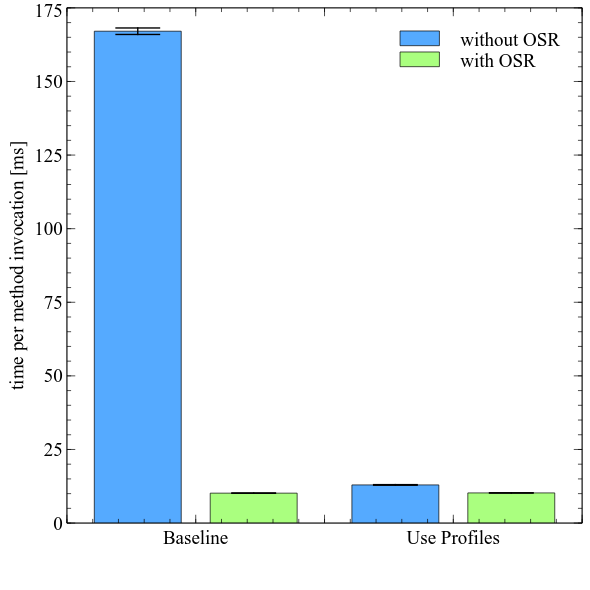
\includegraphics[width=0.5\textwidth]{figures/nocompile.png}
    \caption{NoCompile.method1 - per method invocation time}
    \label{f:nocompile}
  \end{center}
\end{figure}
\\
Enabling OSR again and the difference between with and without cached profiles vanishes.
This happens because Hotspot quickly realizes the hotness of the method and compiles it during the first invocation already. 
Since the method is simple the OSR compiled version already includes enough profiling information and does not trigger any deoptimizations. Therefore there is also no performance difference when using the cached profile.
\subsection{Example 2}
\label{s:ex2}
However, OSR is one of the main features of Hotspot to improve the JIT performance and disabling that does not give us any practical results. Since we want an example which demonstrates the influence of cached profiles, I came up with the example sketched in Listing \ref{l:manydeopts} which is slightly more complex but still easy to understand.
\\\\
The idea is to create a method that takes a different, long running branch on each of it's method invocations. Each branch has been constructed in a way that it will trigger an OSR compilation. When compiling this method during its first iteration only the first branch will be included in the compiled code. The same will happen for each of the 100 method invocations. As one can see in Figure \ref{f:manydeopts} the baseline indeed averages at around 130 deoptimizations and a time per method invocation of 200 ms.
\\\\
Now I use a regular execution to dump the profiles and then use these profiles. So theoretically the profiles dumped after a full execution should include knowledge of all branches and therefore the compiled method using these profiles should not run into any deoptimizations. As one can see in Figure \ref{f:manydeopts} this is indeed the case. When using the cached profiles no more deoptimizations occur and because less time is spent profiling and compiling the methods the per method execution time is even significantly faster with averaging at 190ms now.
\begin{lstlisting}[float,caption=Simple method that causes many deoptimizations,label=l:manydeopts,language=Java]
class ManyDeopts {
    double result = 0.0;
    for(int c = 0; c < 100; c++) {
      result = method1(result);
    }
    public static long method1(long count) {
        for(int k = 0l; k < 10000000l; k++) {
            if (count < 10000000l) {
                count = count + 1;
            } else if (count < 30000000l) {
                count = count + 2;
                .
                .
                .
            } else if (count < 50500000000l) {
               count = count + 100;
            }
            count = count + 50000;
        }
        return count;
   }
}
\end{lstlisting}
\begin{figure}[ht]
  \begin{center}
    \centering
    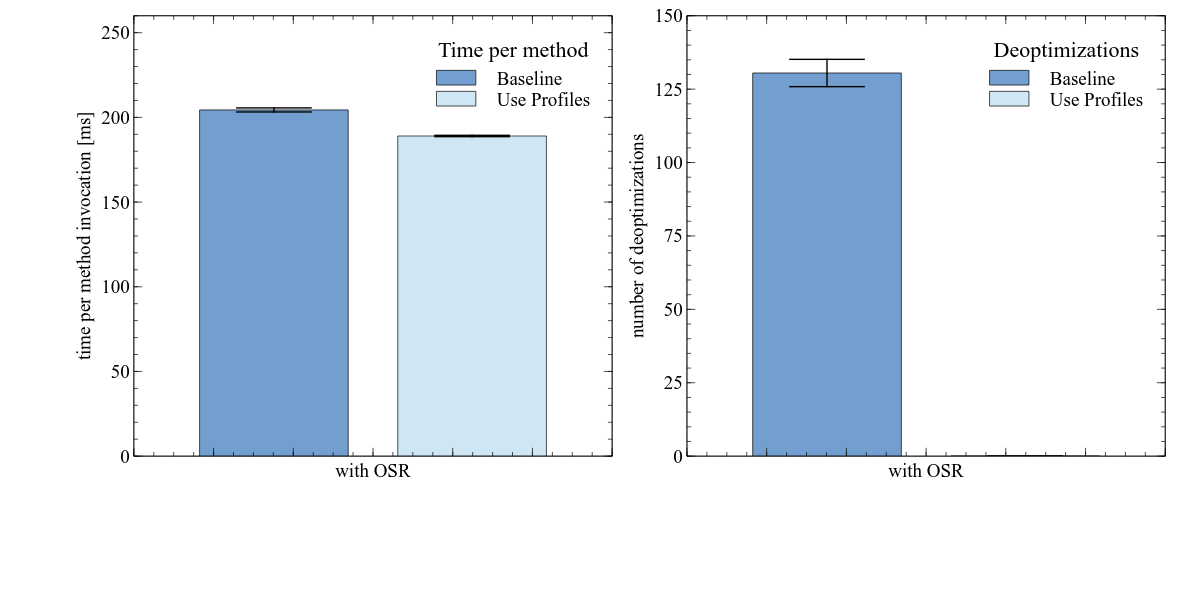
\includegraphics[width=0.9\textwidth]{figures/manydeopt.png}
    \caption{ManyDeopts.method1 - per method invocation time and deoptimization count}
    \label{f:manydeopts}
  \end{center}
\end{figure}
